\documentclass[tikz,border=10pt]{standalone}
\usepackage{amssymb} % For \varnothing symbol
\usetikzlibrary{positioning, shapes.geometric}

\begin{document}
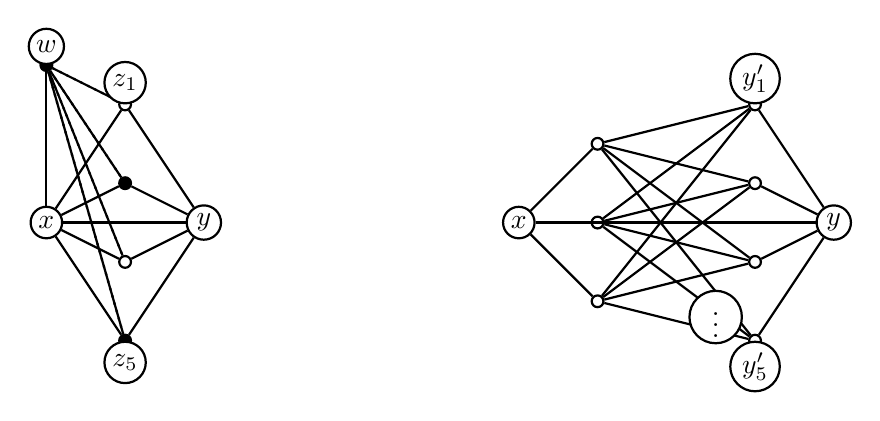
\begin{tikzpicture}[node distance=1.5cm, thick,
    every node/.style={circle, draw, fill=white, inner sep=1.5pt},
    dot/.style={circle, draw, fill=black, inner sep=1.5pt}
]

% LEFT SIDE OF THE IMAGE
\begin{scope}[local bounding box=left_diagram]
    % Nodes
    \node (x) at (0,0) {$x$};
    \node (w) at (0,2) [dot] {};
    \node (z1) at (1,1.5) {};
    \node (z2) at (1,0.5) [dot] {};
    \node (z3) at (1,-0.5) {};
    \node (z4) at (1,-1.5) [dot] {};
    \node (y) at (2,0) {$y$};

    % Edges
    \draw (x) -- (w);
    \draw (x) -- (z1);
    \draw (x) -- (z2);
    \draw (x) -- (z3);
    \draw (x) -- (z4);
    \draw (x) -- (y);
    \draw (w) -- (z1);
    \draw (w) -- (z2);
    \draw (w) -- (z3);
    \draw (w) -- (z4);
    \draw (y) -- (z1);
    \draw (y) -- (z2);
    \draw (y) -- (z3);
    \draw (y) -- (z4);

    % Dotted lines for w-z_i
    \draw[dotted] (w) -- (z1);
    \draw[dotted] (w) -- (z2);
    \draw[dotted] (w) -- (z3);
    \draw[dotted] (w) -- (z4);

    % Labels
    \node[above] at (w) {$w$};
    \node[above] at (z1) {$z_1$};
    \node[below] at (z4) {$z_5$};
\end{scope}

% RIGHT SIDE OF THE IMAGE
\begin{scope}[shift={(6,0)}, local bounding box=right_diagram]
    % Nodes
    \node (x) at (0,0) {$x$};
    \node (x1) at (1,1) {};
    \node (x2) at (1,0) {};
    \node (x3) at (1,-1) {};
    \node (y) at (4,0) {$y$};
    \node (y1) at (3,1.5) {};
    \node (y2) at (3,0.5) {};
    \node (y3) at (3,-0.5) {};
    \node (y4) at (3,-1.5) {};

    % Edges
    \draw (x) -- (x1);
    \draw (x) -- (x2);
    \draw (x) -- (x3);
    \draw (x) -- (y);
    \draw (y) -- (y1);
    \draw (y) -- (y2);
    \draw (y) -- (y3);
    \draw (y) -- (y4);
    \draw (x1) -- (y1);
    \draw (x1) -- (y2);
    \draw (x1) -- (y3);
    \draw (x1) -- (y4);
    \draw (x2) -- (y1);
    \draw (x2) -- (y2);
    \draw (x2) -- (y3);
    \draw (x2) -- (y4);
    \draw (x3) -- (y1);
    \draw (x3) -- (y2);
    \draw (x3) -- (y3);
    \draw (x3) -- (y4);

    % Labels
    \node[above] at (y1) {$y'_1$};
    \node[below] at (y4) {$y'_5$};
    \node at (2.5, -1.2) {$\vdots$};
\end{scope}

\end{tikzpicture}
\end{document}